\documentclass[a4paper, 10pt]{article}
\usepackage[latin1]{inputenc}
\usepackage[T1]{fontenc}
\usepackage[english]{babel}
\usepackage{graphicx}
\usepackage{amsmath}
\usepackage{amssymb}
\usepackage{stmaryrd}
\usepackage{hyperref}
\usepackage{lmodern}

\pagestyle{headings}

\title{Overview of the tool - Graal Stratified Negation}
\author{Boixel Arthur}
\date{\today}

\begin{document}

\maketitle

\begin{abstract}
  This document presents the different functionalities of the Java tool and how to use them in the Graphical User Interface. This is a minimal description of the Graphical User Interface, only the most important functionalities are described.
\end{abstract}

\newpage

\tableofcontents

\newpage
\section{Launch the GUI}
The GUI will start if you launch the tool with the \verb=-w= or \verb=--window= option. No other options are needed.\\
\begin{center}
  \verb= java -jar graal-stratified-negation.jar -w=
\end{center}


\section{Ontology}
The programm works with an ontology.
\subsection{Load}
To load an ontology (in \verb=DLGP= format) from a file, click \verb=Open= on the top left \verb=File= menu of the GUI as shown in Figure \ref{fig1} and select the file that contains your rules.
\begin{figure}
  \begin{center}
    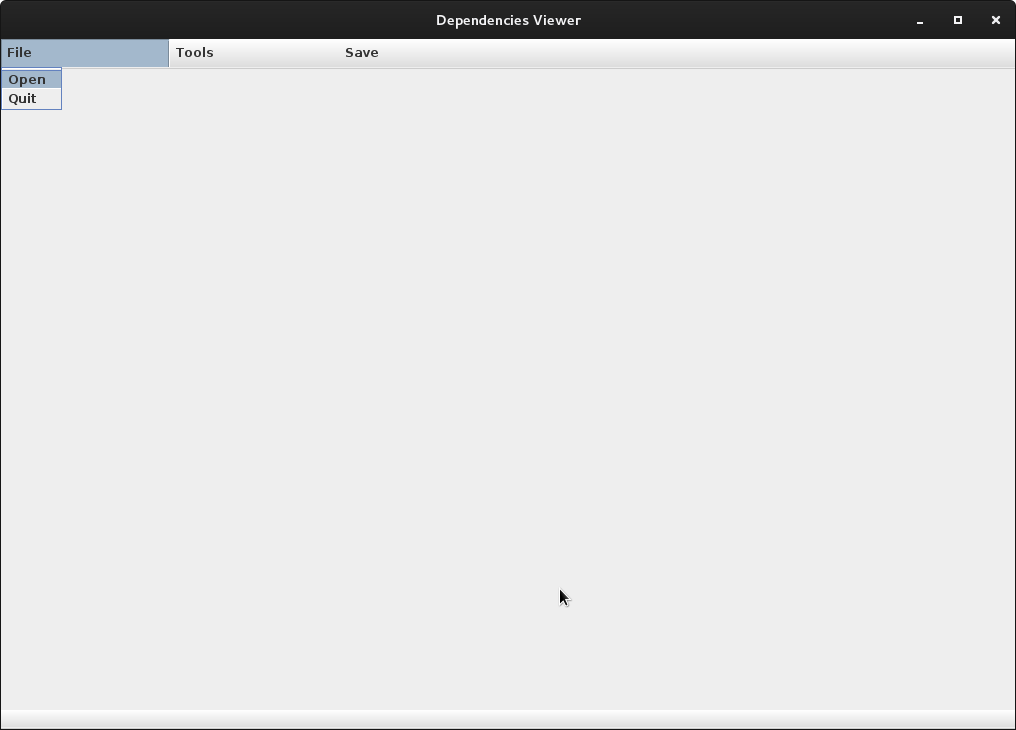
\includegraphics[scale=0.25]{pics/fig1.png}
    \caption{Open an ontology}
  \end{center}
  \label{fig1}
\end{figure}

\subsection{Visualize}
Once you opened an ontology you can visualize the rules by clicking on \verb=Print Rules= in the \verb=Tool= menu as shown in Figure \ref{fig2}.
\begin{figure}
\begin{center}
  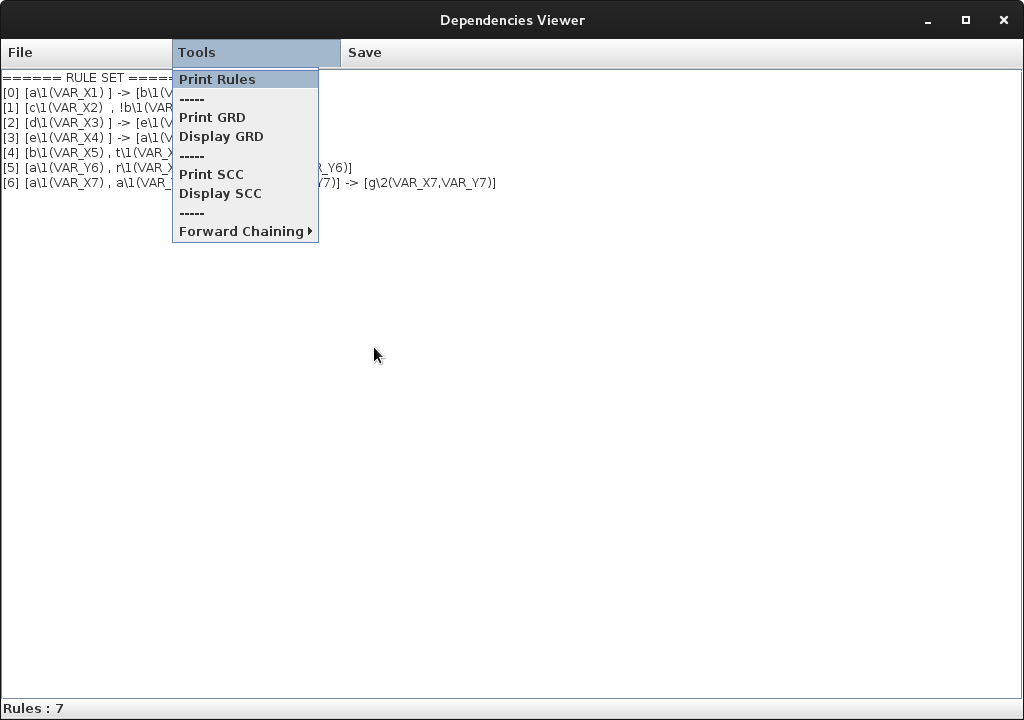
\includegraphics[scale=0.25]{pics/fig2.png}
  \caption{Print rules set}
\end{center}
\label{fig2}
\end{figure}

\subsection{Save}
You can save your labeled ontology into a file by clicking on \verb=Save Rules= in the \verb=Save= menu as shown in Figure \ref{fig3}.
\begin{figure}
\begin{center}
  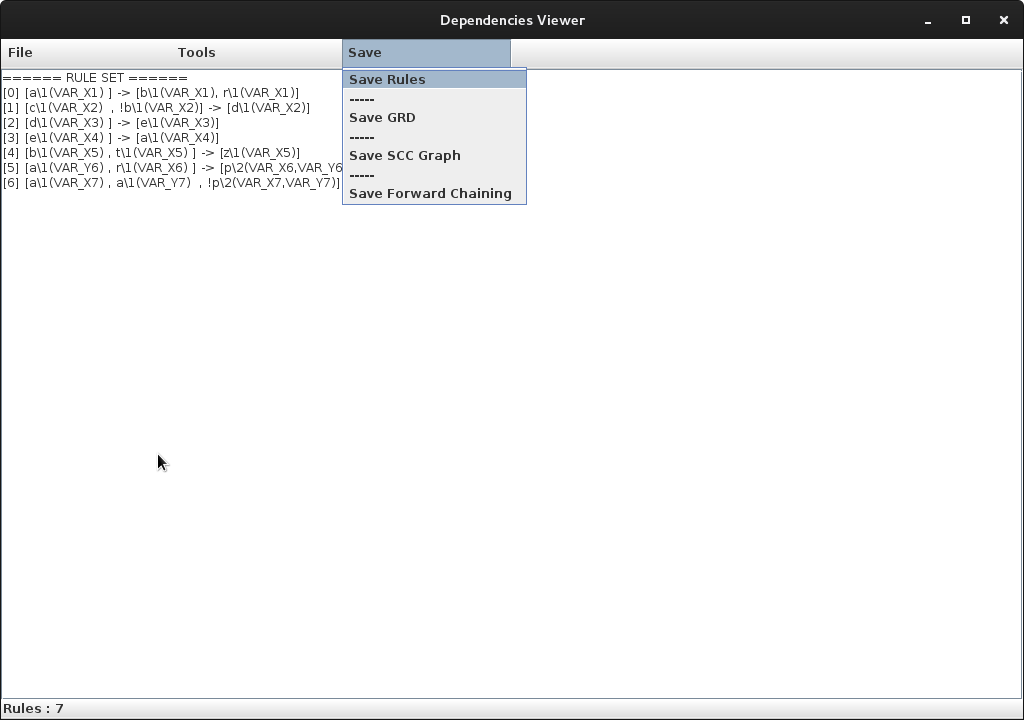
\includegraphics[scale=0.25]{pics/fig3.png}
  \caption{Save rules set}
\end{center}
\label{fig3}
\end{figure}

\newpage

\section{Graph of Rule Dependencies}
Once you opened an ontology the tool will compute its graph of rules dependencies. Please note that this may take some time with big ontologies.
\subsection{Visualize}
There are two ways to visualize the Graph of Rules Dependencies.
\subsubsection{Text}
By clicking on \verb=Print GRD= in the \verb=Tool= menu you will see the text version of the graph as shown in Figure \ref{fig4}. The text version can be used to do some post treatment. In the bottom of the GUI you can see different information about the graph :
\begin{itemize}
\item Number of rules (nodes)
\item Number of dependencies (edges)
\item Wether the ontology can be stratified or not
\end{itemize}

\begin{figure}
  \begin{center}
    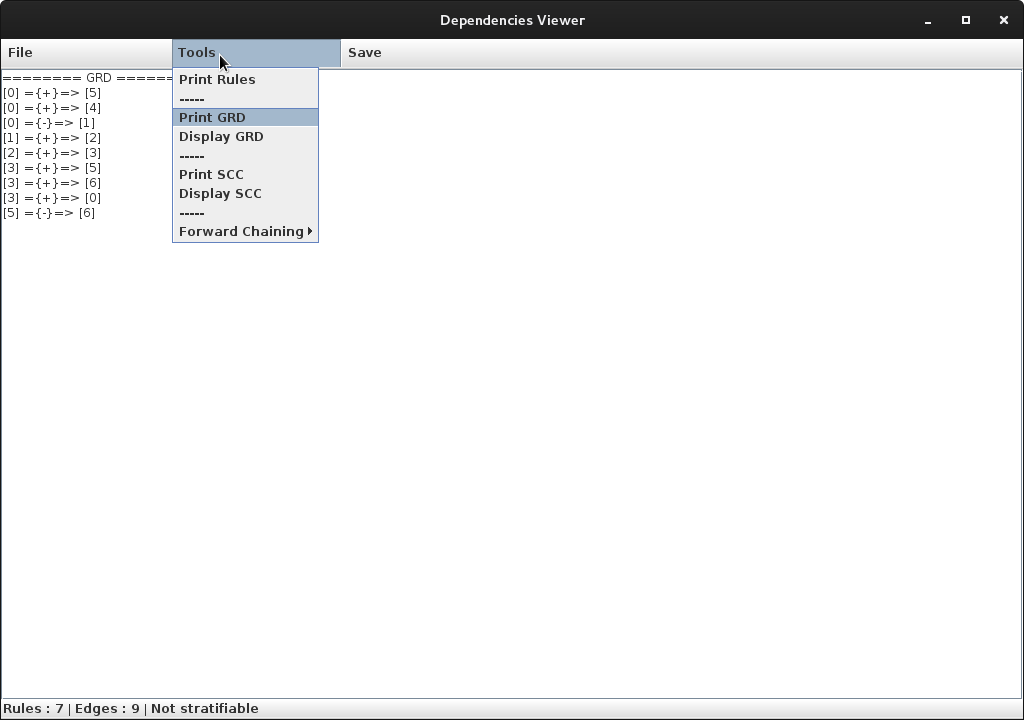
\includegraphics[scale=0.25]{pics/fig4.png}
    \caption{Print GRD}
  \end{center}
  \label{fig4}
\end{figure}

\subsubsection{Graphical}
By clicking on \verb=Display GRD= in the \verb=Tool= menu as shown in Figure \ref{fig5}, you can see a graphical and dynamic representation of the graph.\\
Nodes can be green or red. A red node belongs to a circuit which contains a negative reliance. That means that the set of rules is not stratifiable. If there are only green nodes, the set of rules is stratifiable.\\
Egdes can be black, orange or red. A red edge represents a negative reliance which is part of a circuit : the rule set is not stratifiable. An orange edge represents a negative reliance which does not cause any problem and a black edge represents a positive reliance between two rules.

\begin{figure}
\begin{center}
  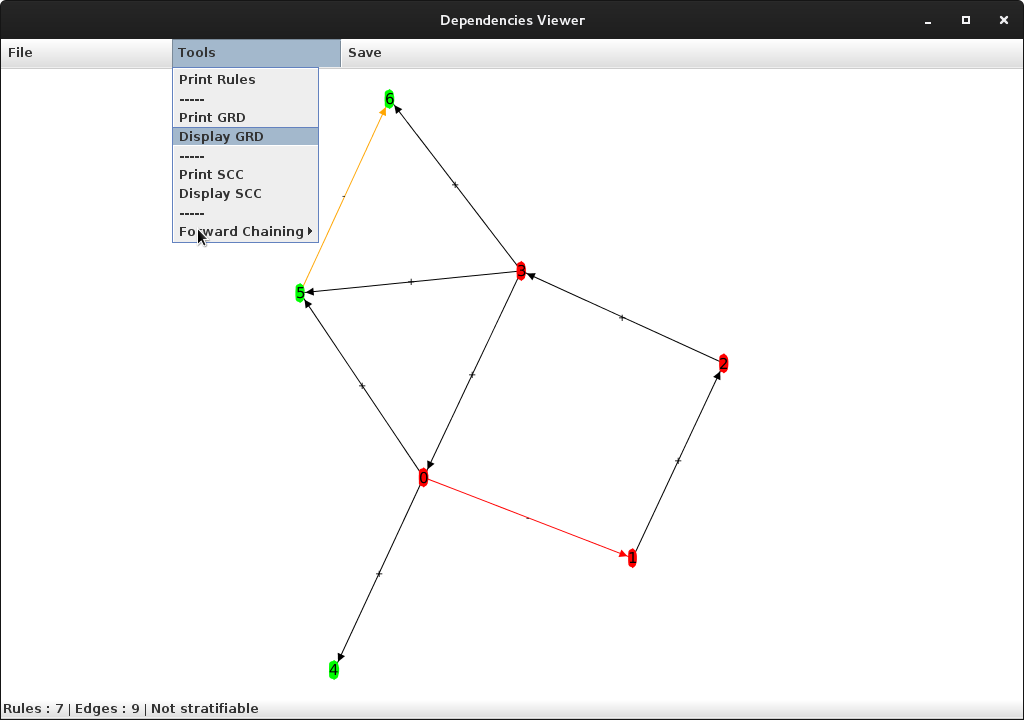
\includegraphics[scale=0.25]{pics/fig5.png}
  \caption{Display GRD}
\end{center}
\label{fig5}
\end{figure}

\subsection{Save}
To make some post treatment of the Graph of Rule Dependencies you can save it to a file by clicking on \verb=Save GRD= in the \verb=Save= menu as shown in Figure \ref{fig6}. The graph will be saved as you can see it when you print it.
\begin{figure}
\begin{center}
  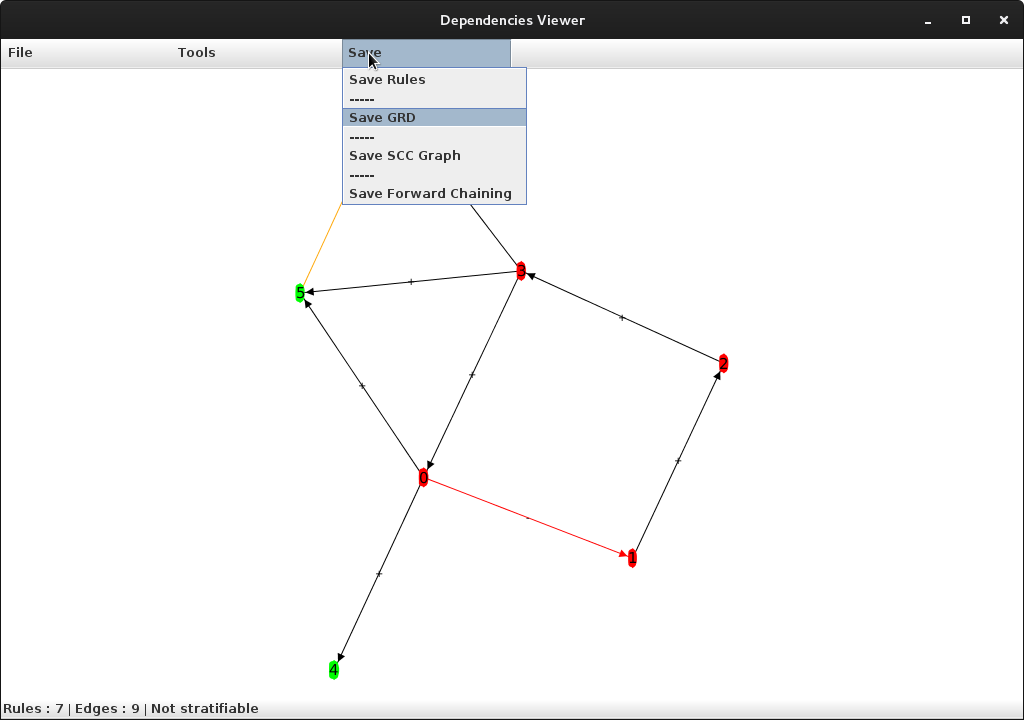
\includegraphics[scale=0.25]{pics/fig6.png}
  \caption{Save GRD}
\end{center}
\label{fig6}
\end{figure}


\newpage

\section{Graph of Strongly Connected Components}
When computing the Graph of Rule Dependencies the tool will automatically compute its Graph of Strongly Connected ComponentS. This graph helps you detect where are the bad circuits in the Graph of Rule Dependencies.

\subsection{Visualize}
There are two ways to visualize it.

\subsubsection{Text}
By clicking on \verb=Print SCC= in the \verb=Tool= menu you will see the text version of the graph as shown in Figure \ref{fig7}. The text version can be used to do some post treatment.
\begin{figure}
\begin{center}
  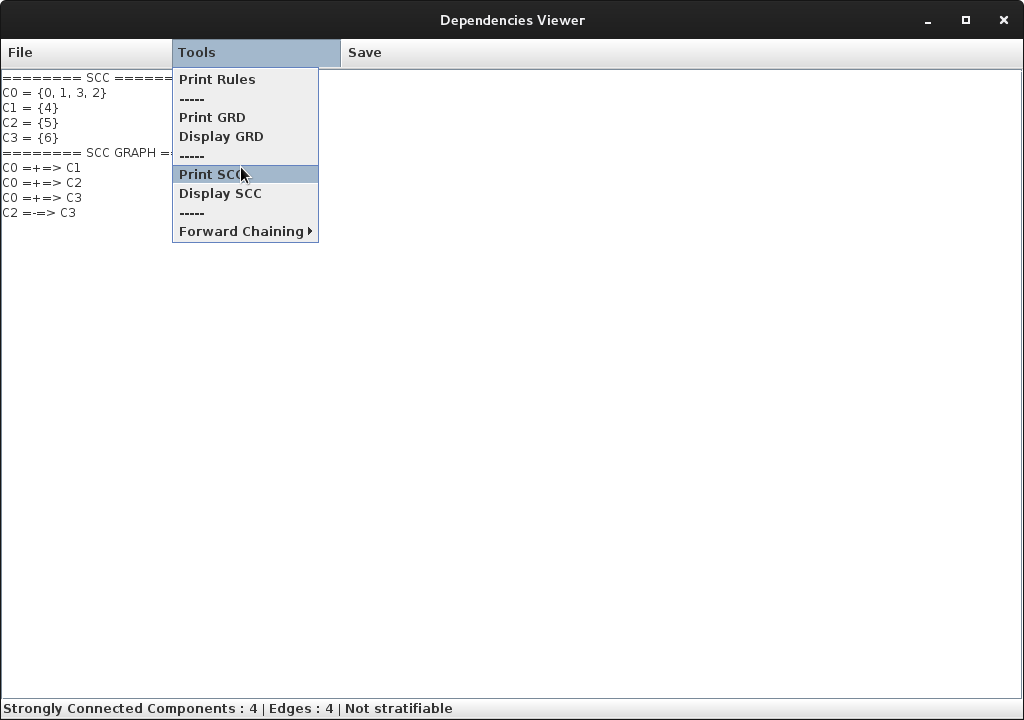
\includegraphics[scale=0.25]{pics/fig7.png}
  \caption{Print SCC}
\end{center}
\label{fig7}
\end{figure}

\subsubsection{Graphical}
By clicking on \verb=Display SCC= in the \verb=Tool= menu as shown in Figure \ref{fig8}, you can see a graphical and dynamic representation of the graph.\\
Nodes can be green or red. A red node is a strongly connected components which contains a circuit with a negative reliance. That means that the set of rules is not stratifiable. By clicking on a node, a new window will display the Graph of Rule Dependencies of the associated strongly connected component. If there are only green nodes, the set of rules is stratifiable.\\
Egdes can be black or orange. An orange edge represents a negative reliance and a black edge represents a positive reliance between to set of rules.
\begin{figure}
\begin{center}
  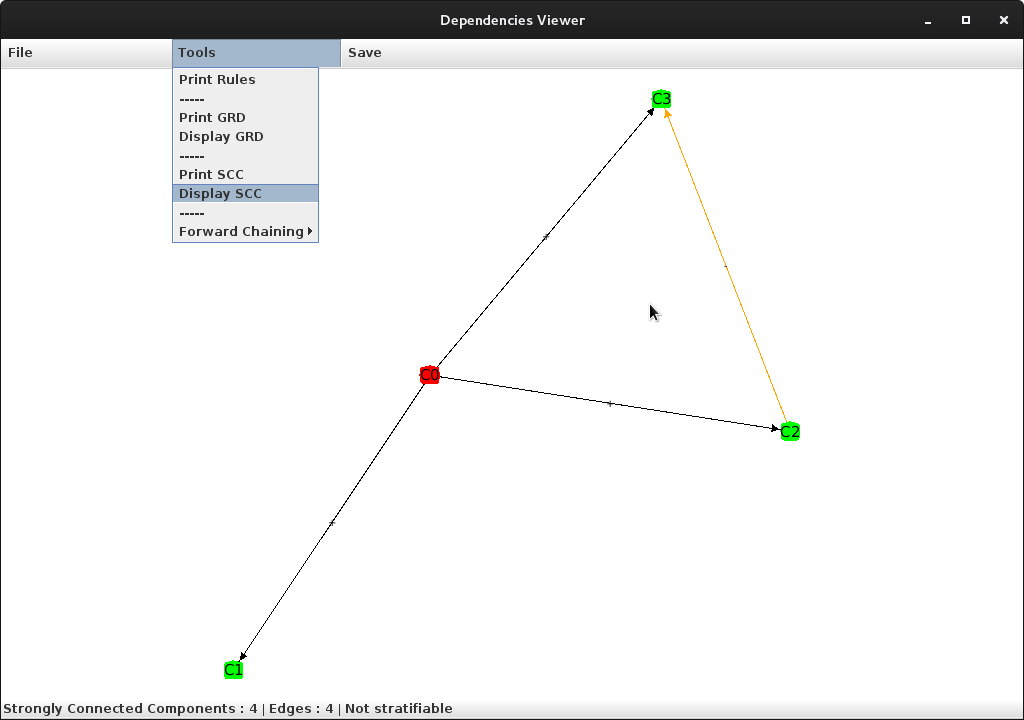
\includegraphics[scale=0.25]{pics/fig8.png}
  \caption{Display SCC}
\end{center}
\label{fig8}
\end{figure}

\subsection{Save}
To make some post treatment on the Graph of Strongly connected Components you can save it to a file by clicking on \verb=Save SCC Graph= in the \verb=Save= menu as shown in Figure \ref{fig9}. The graph will be saved as you can see it when you print it.
\begin{figure}
\begin{center}
  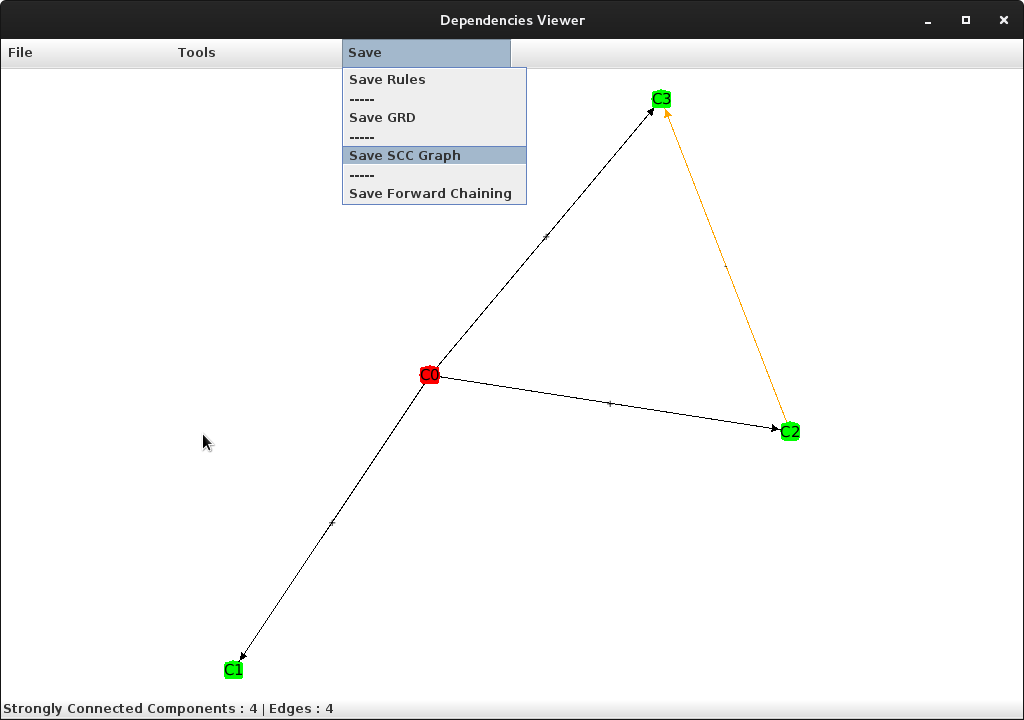
\includegraphics[scale=0.25]{pics/fig9.png}
  \caption{Save SCC Graph}
\end{center}
\label{fig9}
\end{figure}

\newpage

\section{Forward Chaining}
If your set of rules is stratifiable you can apply the forward chaining mechanism on a set of facts (the forward chaining will use the computed stratification).
\subsection{Execute}
\subsubsection{From a file}
By clicking on \verb=From file= in the \verb=Forward Chaining= submenu of the \verb=Tool= menu, you can select a file which contain your set of facts. The tool will apply the forward chaining mechanism and print the result as shown for example in Figure \ref{fig10}.
\begin{figure}
\begin{center}
  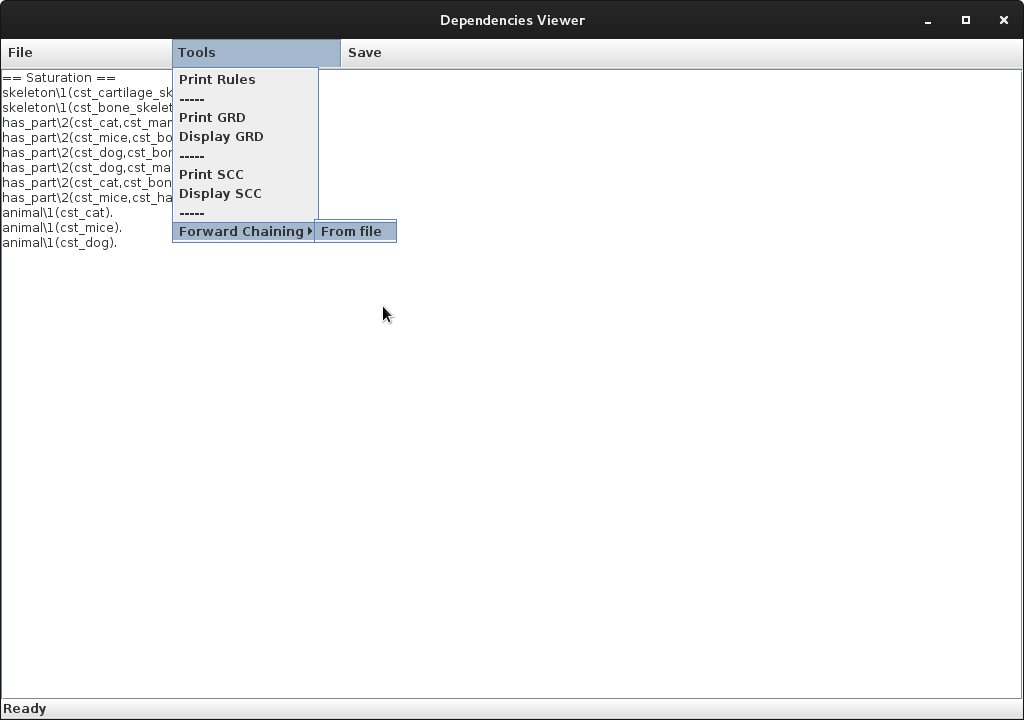
\includegraphics[scale=0.25]{pics/fig10.png}
  \caption{Forward Chaining Application}
\end{center}
\label{fig10}
\end{figure}

\subsection{Save}
By clicking on \verb=Save Forward Chaining= in the \verb=Save= menu as shown in Figure \ref{fig11} you can save a saturated fact base. You can select a file in which the tool will save the result of the forward chaining execution on a specified file of facts.
\begin{figure}
\begin{center}
  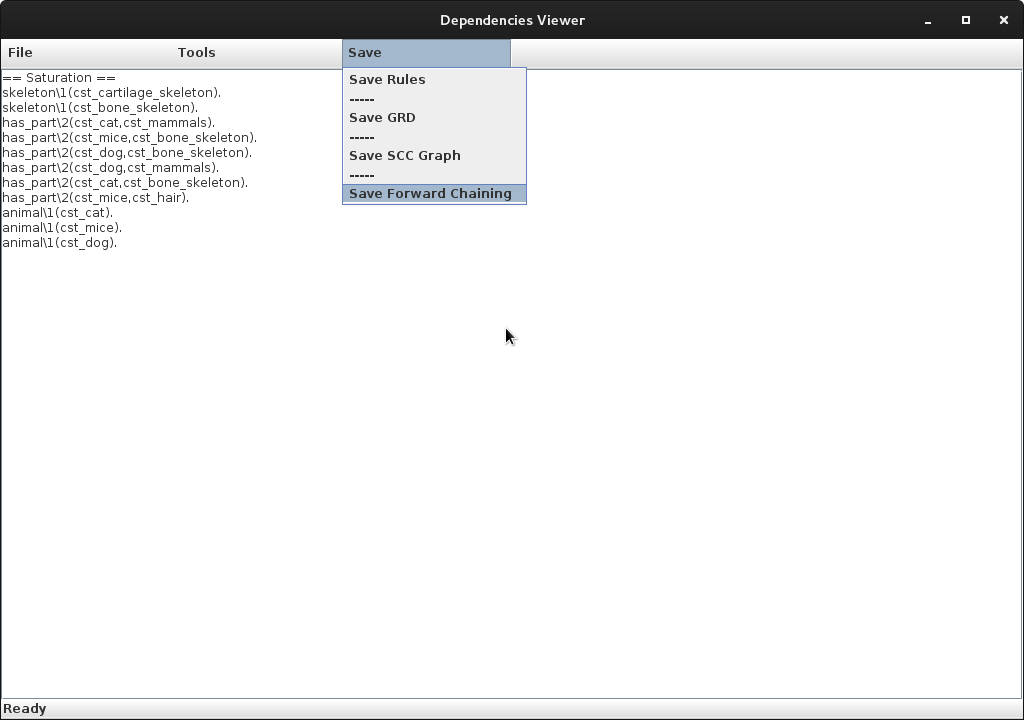
\includegraphics[scale=0.25]{pics/fig11.png}
  \caption{Save Forward Chaining}
\end{center}
\label{fig11}
\end{figure}

\end{document}

